

\tikzset{every picture/.style={line width=0.75pt}} %set default line width to 0.75pt        

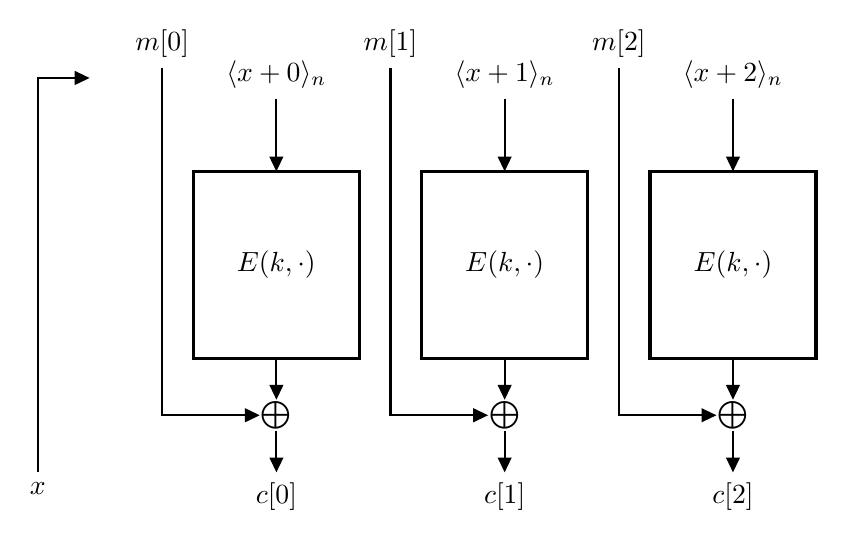
\begin{tikzpicture}[x=0.75pt,y=0.75pt,yscale=-1,xscale=1]
%uncomment if require: \path (0,262); %set diagram left start at 0, and has height of 262

%Shape: Rectangle [id:dp9182651949275114] 
\draw  [line width=1.2]  (90,80) -- (170,80) -- (170,170) -- (90,170) -- cycle ;
%Straight Lines [id:da8170265303379278] 
\draw    (130,45) -- (130,77) ;
\draw [shift={(130,80)}, rotate = 270] [fill={rgb, 255:red, 0; green, 0; blue, 0 }  ][line width=0.08]  [draw opacity=0] (7.14,-3.43) -- (0,0) -- (7.14,3.43) -- cycle    ;
%Straight Lines [id:da42259864047214935] 
\draw    (130.03,170) -- (130.03,187) ;
\draw [shift={(130.03,190)}, rotate = 270] [fill={rgb, 255:red, 0; green, 0; blue, 0 }  ][line width=0.08]  [draw opacity=0] (7.14,-3.43) -- (0,0) -- (7.14,3.43) -- cycle    ;
%Shape: Rectangle [id:dp621298686621194] 
\draw  [line width=1.2]  (200,80) -- (280,80) -- (280,170) -- (200,170) -- cycle ;
%Straight Lines [id:da34503563282164884] 
\draw    (240,45) -- (240,77) ;
\draw [shift={(240,80)}, rotate = 270] [fill={rgb, 255:red, 0; green, 0; blue, 0 }  ][line width=0.08]  [draw opacity=0] (7.14,-3.43) -- (0,0) -- (7.14,3.43) -- cycle    ;
%Shape: Rectangle [id:dp9795216608775008] 
\draw  [line width=1.2]  (310,80) -- (390,80) -- (390,170) -- (310,170) -- cycle ;
%Straight Lines [id:da21108705765109503] 
\draw    (350,45) -- (350,77) ;
\draw [shift={(350,80)}, rotate = 270] [fill={rgb, 255:red, 0; green, 0; blue, 0 }  ][line width=0.08]  [draw opacity=0] (7.14,-3.43) -- (0,0) -- (7.14,3.43) -- cycle    ;
%Straight Lines [id:da15378402713059036] 
\draw    (130.03,205) -- (130.03,222) ;
\draw [shift={(130.03,225)}, rotate = 270] [fill={rgb, 255:red, 0; green, 0; blue, 0 }  ][line width=0.08]  [draw opacity=0] (7.14,-3.43) -- (0,0) -- (7.14,3.43) -- cycle    ;
%Straight Lines [id:da30531935370310403] 
\draw    (240,170) -- (240,187) ;
\draw [shift={(240,190)}, rotate = 270] [fill={rgb, 255:red, 0; green, 0; blue, 0 }  ][line width=0.08]  [draw opacity=0] (7.14,-3.43) -- (0,0) -- (7.14,3.43) -- cycle    ;
%Straight Lines [id:da24126879345014207] 
\draw    (240,205) -- (240,222) ;
\draw [shift={(240,225)}, rotate = 270] [fill={rgb, 255:red, 0; green, 0; blue, 0 }  ][line width=0.08]  [draw opacity=0] (7.14,-3.43) -- (0,0) -- (7.14,3.43) -- cycle    ;
%Straight Lines [id:da37363638556457834] 
\draw    (350,170) -- (350,187) ;
\draw [shift={(350,190)}, rotate = 270] [fill={rgb, 255:red, 0; green, 0; blue, 0 }  ][line width=0.08]  [draw opacity=0] (7.14,-3.43) -- (0,0) -- (7.14,3.43) -- cycle    ;
%Straight Lines [id:da33550574981005155] 
\draw    (350,205) -- (350,222) ;
\draw [shift={(350,225)}, rotate = 270] [fill={rgb, 255:red, 0; green, 0; blue, 0 }  ][line width=0.08]  [draw opacity=0] (7.14,-3.43) -- (0,0) -- (7.14,3.43) -- cycle    ;
%Straight Lines [id:da7787352563430161] 
\draw    (75,30) -- (75,197.5) -- (119,197.5) ;
\draw [shift={(122,197.5)}, rotate = 180] [fill={rgb, 255:red, 0; green, 0; blue, 0 }  ][line width=0.08]  [draw opacity=0] (7.14,-3.43) -- (0,0) -- (7.14,3.43) -- cycle    ;
%Straight Lines [id:da27942679319004915] 
\draw    (185,30) -- (185,197.5) -- (229,197.5) ;
\draw [shift={(232,197.5)}, rotate = 180] [fill={rgb, 255:red, 0; green, 0; blue, 0 }  ][line width=0.08]  [draw opacity=0] (7.14,-3.43) -- (0,0) -- (7.14,3.43) -- cycle    ;
%Straight Lines [id:da2614954421927662] 
\draw    (295,30) -- (295,197.5) -- (339,197.5) ;
\draw [shift={(342,197.5)}, rotate = 180] [fill={rgb, 255:red, 0; green, 0; blue, 0 }  ][line width=0.08]  [draw opacity=0] (7.14,-3.43) -- (0,0) -- (7.14,3.43) -- cycle    ;
%Straight Lines [id:da5245035261811899] 
\draw    (37,35) -- (15,35) -- (15,225) ;
\draw [shift={(40,35)}, rotate = 180] [fill={rgb, 255:red, 0; green, 0; blue, 0 }  ][line width=0.08]  [draw opacity=0] (7.14,-3.43) -- (0,0) -- (7.14,3.43) -- cycle    ;

% Text Node
\draw (130,125) node    {$E( k,\cdot )$};
% Text Node
\draw (75,26.6) node [anchor=south] [inner sep=0.75pt]    {$m[ 0]$};
% Text Node
\draw (130.03,228.4) node [anchor=north] [inner sep=0.75pt]    {$c[ 0]$};
% Text Node
\draw (240,125) node    {$E( k,\cdot )$};
% Text Node
\draw (185,26.6) node [anchor=south] [inner sep=0.75pt]    {$m[ 1]$};
% Text Node
\draw (240,228.4) node [anchor=north] [inner sep=0.75pt]    {$c[ 1]$};
% Text Node
\draw (350,125) node    {$E( k,\cdot )$};
% Text Node
\draw (295,26.6) node [anchor=south] [inner sep=0.75pt]    {$m[ 2]$};
% Text Node
\draw (350,228.4) node [anchor=north] [inner sep=0.75pt]    {$c[ 2]$};
% Text Node
\draw (130,197.5) node    {$\bigoplus $};
% Text Node
\draw (240,197.5) node    {$\bigoplus $};
% Text Node
\draw (350,197.5) node    {$\bigoplus $};
% Text Node
\draw (130,41.6) node [anchor=south] [inner sep=0.75pt]    {$\langle x+0\rangle _{n}$};
% Text Node
\draw (240,41.6) node [anchor=south] [inner sep=0.75pt]    {$\langle x+1\rangle _{n}$};
% Text Node
\draw (350,41.6) node [anchor=south] [inner sep=0.75pt]    {$\langle x+2\rangle _{n}$};
% Text Node
\draw (15,228.4) node [anchor=north] [inner sep=0.75pt]    {$x$};


\end{tikzpicture}